\documentclass{article}

% If you're new to LaTeX, here's some short tutorials:
% https://www.overleaf.com/learn/latex/Learn_LaTeX_in_30_minutes
% https://en.wikibooks.org/wiki/LaTeX/Basics

% Formatting
\usepackage[utf8]{inputenc}
\usepackage[margin=1in]{geometry}
\usepackage[titletoc,title]{appendix}

% Math
% https://www.overleaf.com/learn/latex/Mathematical_expressions
% https://en.wikibooks.org/wiki/LaTeX/Mathematics
\usepackage{amsmath,amsfonts,amssymb,mathtools}

% Images
% https://www.overleaf.com/learn/latex/Inserting_Images
% https://en.wikibooks.org/wiki/LaTeX/Floats,_Figures_and_Captions
\usepackage{graphicx,float}

% Tables
% https://www.overleaf.com/learn/latex/Tables
% https://en.wikibooks.org/wiki/LaTeX/Tables

% Algorithms
% https://www.overleaf.com/learn/latex/algorithms
% https://en.wikibooks.org/wiki/LaTeX/Algorithms
\usepackage[ruled,vlined]{algorithm2e}
\usepackage{algorithmic}

% Code syntax highlighting
% https://www.overleaf.com/learn/latex/Code_Highlighting_with_minted
\usepackage{minted}
\usemintedstyle{borland}

% References
% https://www.overleaf.com/learn/latex/Bibliography_management_in_LaTeX
% https://en.wikibooks.org/wiki/LaTeX/Bibliography_Management
\usepackage{biblatex}
\addbibresource{references.bib}

% Title content
\title{NI-KOP Homework 1}
\author{Patrik Jantošovič}
\date{October 11, 2020}

\begin{document}

\maketitle

\section{The Decision Version Of Knapsack Problem}
The given is integer n as number of items, integer M as the capacity of the knapsack, integer B as minimal price of the knapsack and two finite sets W and C. W=$\{w_1, .., w_n\}$ being the set of weights of items and C=$\{c_1, .., c_n\}$ being the set of costs of items. The task is then to decide if it is possible to construct a finite set X=$\{x_1, ..., x_n\}$ where each $x_i$ is either 0 or 1 so that:
\begin{equation}
    w_1x_1 + w_2x_2 + ... + w_nx_n<= M
\end{equation}
\begin{equation}
    c_1x_1 + c_2x_2 + ... + c_nx_n >= B
\end{equation}

\section{Implementation}
JAVA implementation was created to solve this problem and cross-checked with provided solutions. I managed to implement both a decision and constructive algorithm, difference being in stopping the algorithm once we decide we can not reach the minimal price in decision version of the problem. Which obviously does not apply to constructive version of the problem as we want to reach maximum possible price every time.
\\
\\
I also created a simple powershell script that was used to run the application somewhat automatically.
\\
\\
The full implementation can be viewed here: https://github.com/PatrikJantosovic/NI-KOP-Homeworks

\subsection{BruteForce Algorithm}
Using the powerset idea \cite{pwset}, the main code looks like this:
\inputminted{java}{bf.java}

\subsection{Branch\&Bound Algorithm}
For branch and bound solution, recursive approach was selected. The algorithm is actually very similar as running the brute-force recursively generates a whole tree, but by adding the following conditions we can cut some branches:
\inputminted{java}{bb.java}

\section{Results}
Tests were run on Windows 10 64bit machine, with AMD Ryzen 7 PRO 2700U and Radeon Vega Mobile Gfx. Two data sets NR and ZR were provided and have been evaluated separately as requested.

\subsection{NR Data Set}
Looking at the computational time, we can see significant differences in the algorithms. In the Figure 1 we can see BF (blue) line being the Brute-Force algorithm and BB(orange) line being the Branch and Bound algorithm.
\\
\\
Figure 2 shows us that while computational complexity of Branch\&Bound is smaller than the Brute-Force, the number of visited node grows exponentially depending on N. 
\\
\\
The histogram (Figure 3) was created for 10 items. It shows that most of the \textit{cutting} has happened at the start, which shows that there are a lot of instances when minimum price cannot be reached at all. Also, apparently, there are lot of instances when \textit{cutting} occurred at the end or did not occur at all and whole tree was generated.
\begin{figure}[H]
    \centering
    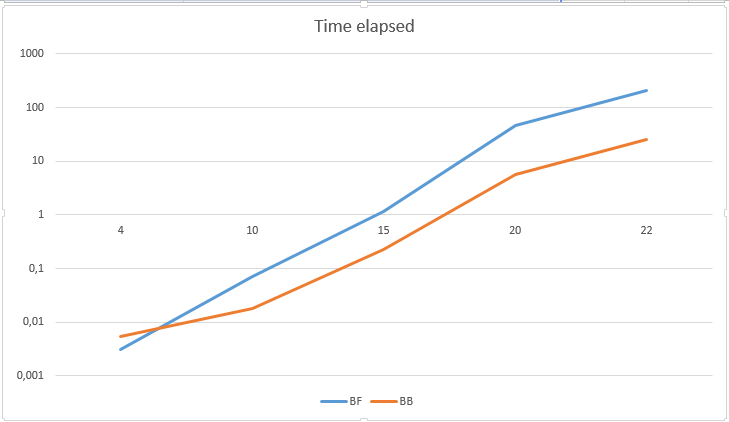
\includegraphics[width=0.8\linewidth]{NRtime.PNG}
    \caption{Time elapsed for NR data set (in seconds)}
\end{figure}
\begin{figure}[H]
    \centering
    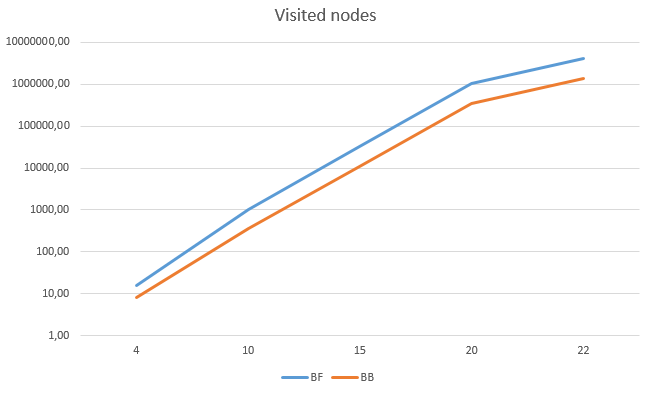
\includegraphics[width=0.8\linewidth]{NRpass.PNG}
    \caption{Average Computational complexity of NR data set (in nodes visited) for given N}
\end{figure}
\begin{figure}[H]
    \centering
    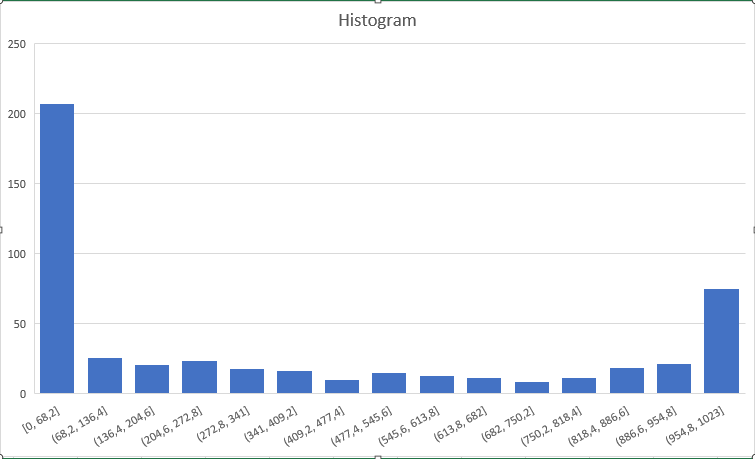
\includegraphics[width=0.8\linewidth]{NRhistogram.PNG}
    \caption{Histogram of NR data set for N=10 }
\end{figure}

\subsection{ZR Data Set}
Not surprisingly, maliciously generated set caused Branch\&Bound algorithm to perform worse, both in computation complexity (Figure 5) and time (Figure 4).
\\
\\
Moreover, the histogram (Figure 6) shows that the decrease in performance is caused by inability to perform branch cutting effectively. Please note, that the histogram starts at \textbf{745}!

\begin{figure}[H]
    \centering
    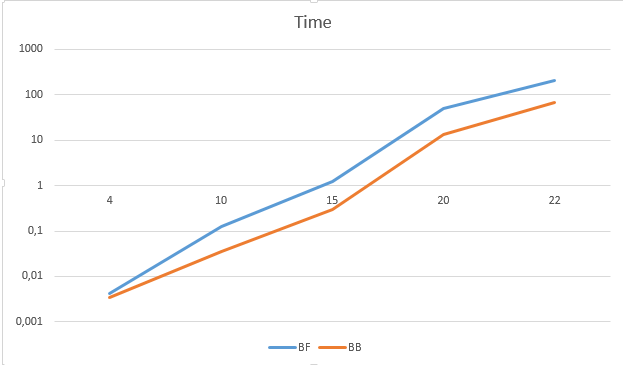
\includegraphics[width=0.8\linewidth]{ZRtime.PNG}
    \caption{Time elapsed for ZR data set (in seconds)}
\end{figure}
\begin{figure}[H]
    \centering
    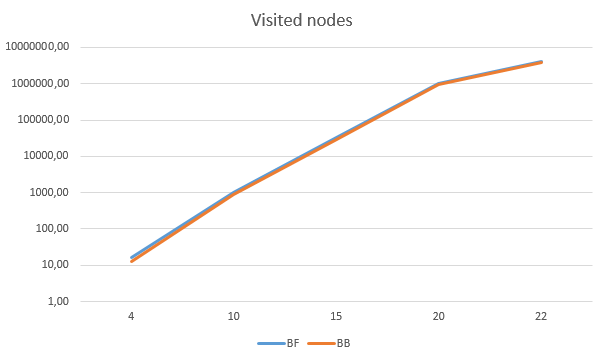
\includegraphics[width=0.8\linewidth]{ZRpass.PNG}
    \caption{Average computational complexity of ZR data set (in nodes visited) for given N}
\end{figure}
\begin{figure}[H]
    \centering
    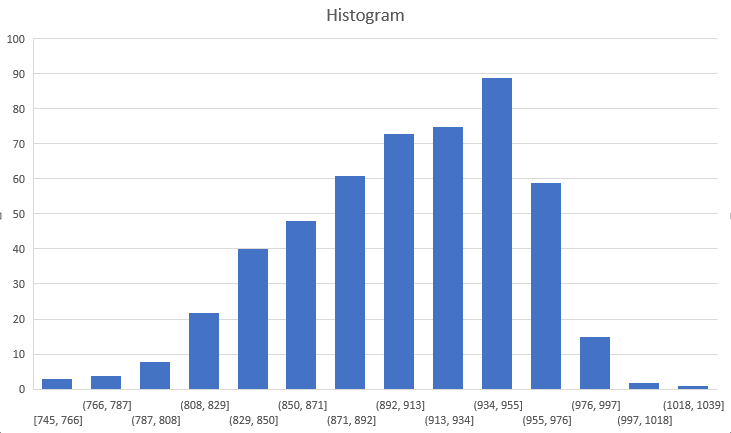
\includegraphics[width=0.8\linewidth]{ZRhistogram.PNG}
    \caption{Histogram of ZR data set for N=10 }
\end{figure}

\subsection{Maximum Complexity}
This subsection is added as I forgot to publish the results of maximum computational complexity on both data sets NR and ZR. The tables show that in the worst case scenario (maximum visited nodes for instance of N), Branch\&Bound behaves exactly like Brute-Force algorithm and the number of nodes visited is $2^N$ on NR data set. Slight improvement was surprisingly seen on ZR data set. Table was intentionally chosen instead of graph as the difference is too small to be visible on graph.
\begin{center}
 \begin{tabular}{||c c c c||} 
 \hline
 N & Branch\&Bound NR & Branch\&Bound ZR & Brute-Force \\ [0.5ex] 
 \hline\hline
 4 & 15 & 16 & 16 \\ 
 \hline
 10 & 1023 & 1019 & 1024 \\
 \hline
 15 & 32767 & 31956 & 32768 \\
 \hline
 20 & 1048575 & 1018174 & 1048576 \\
 \hline \hline
\end{tabular}
\end{center}

% Summary and Conclusions
\section{Summary and Conclusions}
As we observed, while computation complexity was only three times better on random sets (NR) and stayed exponentially dependent on N, Branch\&Bound algorithm performed much better as it was able to cut the computational time significantly.

By comparing the two data sets (NR and ZR), we observed that maliciously generated set (ZR) caused Branch\&Bound algorithm to perform almost as bad as Brute Force algorithm when looking at the computational complexity (number of visited nodes). This is clearly seen on histogram of ZR data set (Figure 6), as all of the \textit{cutting of the branches} happened at the end or did not happen at all. 

% References
\printbibliography

\end{document}
